%% LyX 2.3.6 created this file.  For more info, see http://www.lyx.org/.
%% Do not edit unless you really know what you are doing.
\documentclass[english,aspectratio=169]{beamer}
\usepackage{lmodern}
\renewcommand{\sfdefault}{lmss}
\renewcommand{\ttdefault}{lmtt}
\usepackage[T1]{fontenc}
\usepackage[latin9]{inputenc}
\setlength{\parskip}{\medskipamount}
\setlength{\parindent}{0pt}
\usepackage{babel}
\usepackage{textcomp}
\usepackage{amssymb}
\usepackage{graphicx}
\PassOptionsToPackage{normalem}{ulem}
\usepackage{ulem}
\ifx\hypersetup\undefined
  \AtBeginDocument{%
    \hypersetup{unicode=true}
  }
\else
  \hypersetup{unicode=true}
\fi

\makeatletter

%%%%%%%%%%%%%%%%%%%%%%%%%%%%%% LyX specific LaTeX commands.
\pdfpageheight\paperheight
\pdfpagewidth\paperwidth

%% Because html converters don't know tabularnewline
\providecommand{\tabularnewline}{\\}

%%%%%%%%%%%%%%%%%%%%%%%%%%%%%% Textclass specific LaTeX commands.
% this default might be overridden by plain title style
\newcommand\makebeamertitle{\frame{\maketitle}}%
% (ERT) argument for the TOC
\AtBeginDocument{%
  \let\origtableofcontents=\tableofcontents
  \def\tableofcontents{\@ifnextchar[{\origtableofcontents}{\gobbletableofcontents}}
  \def\gobbletableofcontents#1{\origtableofcontents}
}

%%%%%%%%%%%%%%%%%%%%%%%%%%%%%% User specified LaTeX commands.
%\usetheme{CambridgeUS}
%\usetheme{Singapore}
\usetheme{Warsaw}
\usecolortheme{beaver}
\hypersetup{pdfpagemode=None}
\usepackage{tikz}
\usepackage{color}
\usepackage{listings}
\usepackage{multicol}
\setbeamertemplate{footline}[frame number]

\makeatother

\begin{document}
\title[ESS methods]{Methods in Earth System Science}
\author{Marcello Vichi}
\institute[UCT]{Department of Oceanography\\University of Cape Town\\marcello.vichi@uct.ac.za}
\date{SEA2004F}
\makebeamertitle

\section*{Outline}
\begin{frame}{Outline of the Course}

\begin{multicols}{2}\tableofcontents{}\end{multicols}
\end{frame}


\section{Introduction to ESS}

\subsection{Scales and processes}

\frame{\subsectionpage}

\begin{frame}{The ocean in the Earth system}

\begin{columns}[c]

\column{8cm}

\includegraphics[height=0.7\paperheight]{figures/interactions}

\column{4cm}

An overview of the process and interactions at play in the Earth system.
The white boxes indicate the compartments and the arrow the drivers
and possible changes due to natural and anthropogenic processes. (from
the IPCC Assessment Report 4) 
\end{columns}

\end{frame}
%
\begin{frame}{Earth System Science: interdisciplinary subjects}

\begin{itemize}
\item <1->{\small{}ESS moves beyond the study of Earth in terms of sectoral
disciplines specific for the atmosphere, hydrosphere, cryosphere and
biosphere. It stems from disciplinary knowledge and requires inter-disciplinary
familiarity with}{\small\par}
\begin{itemize}
\item <1->{\small{}Physics and mathematics}{\small\par}
\item <1->{\small{}Chemistry, biology and geology}{\small\par}
\item <1->{\small{}Computer science}{\small\par}
\item <1->{\small{}Economics and social sciences}{\small\par}
\end{itemize}
\item <2->{\small{}The Earth is a }\textbf{\small{}biotic}{\small{} environment
that cannot be separated from its }\textbf{\small{}abiotic}{\small{}
counterpart. The presence of life on Earth has determined the chemical
composition of the environment where life \textquotedblleft lives\textquotedblright{}
today. }{\small\par}
\item <3->{\small{}Biogeochemistry is a fundamental part of ESS. It studies
the cycles of chemical elements in natural systems}{\small\par}
\item <4->\textbf{\small{}ESS is a quantitative science}{\small{}. Conceptual
explanations are always supported by quantitative relationships}{\small\par}
\end{itemize}
\end{frame}
%
\begin{frame}{The contemporary Earth System}

\includegraphics[height=0.7\paperheight]{figures/An-updated-conceptual-model-of-the-Earth-System_W640}

An updated conceptual model of the Earth System (Steffen et al., 2020) 
\end{frame}

\begin{frame}{Experimenting with the Earth}
\begin{itemize}
\item <1->The Earth is as a single dynamic entity with tight linkages between
the physical environment, the non-living chemical elements and the
living components.
\item <2->It is a ``special'' science like astrophysics. We are unable
to perform controlled \textbf{experiments on the planet as a whole}
and then observe the results: we need a \emph{combination of observations
and models} (theoretical and numerical). 
\item <3->We must familiarize with quantitative tools and methods to describe,
understand, and predict these processes
\item <4->We combine several physical and biogeochemical principles to
understand the functioning of the Earth as a system. These processes
occur at multiple temporal and spatial scales
\end{itemize}
\end{frame}

\begin{frame}{Multiple scales}

\begin{columns}[t]

\column{7cm }

\includegraphics[width=7cm]{figures/Met_space_time_scale}

{\footnotesize{}Main scales of atmospheric motion. The weather varies
at the synoptic scale (>days and >100 km). }{\footnotesize\par}

\column{6cm}

\includegraphics[width=6.5cm]{figures/fmars-06-00393-g001}

{\footnotesize{}This figure from }{\footnotesize{}\uline{\href{https://www.frontiersin.org/articles/10.3389/fmars.2019.00393/full}{Benway et al., 2019}}}{\footnotesize{}
shows the multiple scales that are present in the marine system.}{\footnotesize\par}
\end{columns}

\end{frame}

\begin{frame}{Scales and processes}

\begin{columns}[t]

\column{9cm }
\begin{center}
\includegraphics[width=4cm]{figures/fmars-06-00393-g001}\vspace{-0.5cm}
\par\end{center}
\begin{itemize}
\item {\scriptsize{}Biological processes in the marine system are distributed
at various scales. For instance, photosynthesis occurs within phytoplankton
cells in a few seconds but blooms are visible at spatial scales of
more than 100 km and may persist for several days. }{\scriptsize\par}
\item {\scriptsize{}In the shelf region we observe changes in chlorophyll
concentration from space that span 3 orders of magnitude, with a clear
presence of filaments that indicate physical and biological processes
occurring at smaller scales.}{\scriptsize\par}
\end{itemize}

\column{6cm}

\includegraphics[width=5cm]{figures/benguela_OLCI_BLOOMS_17_A_LRG}
\end{columns}

\end{frame}

\begin{frame}{Microbial processes}

\begin{columns}[c]

\column{6cm }

\includegraphics[width=6cm]{figures/SEM-images-showing-examples-of-the-rich-microbial-community-on-PMD-a-pennate-diatom-on}

\column{6cm}
\begin{itemize}
\item {\footnotesize{}The most relevant biogeochemical processes in the
marine system are found at the microbial scale. A dense microbial
community can have a substantial effect on the cycling of nutrients,
can affect the vertical distribution of light and hence the energy
storage in the upper layer of the ocean. }{\footnotesize\par}
\item {\footnotesize{}The }\textbf{\footnotesize{}microbiome}{\footnotesize{}
in the ocean is exposed to continuously varying conditions. It responds
both at individual and system levels by adjusting physiological rates
and behaviours, ultimately modifying the properties of the environment
itself.}{\footnotesize\par}
\end{itemize}
\end{columns}

\end{frame}

\begin{frame}{An interconnected ocean}

\begin{columns}[t]

\column{6cm }
\begin{itemize}
\item {\footnotesize{}The microscale and the larger scales are connected
by the }\textbf{\footnotesize{}physical processes of the dynamical
ocean}{\footnotesize{}. }{\footnotesize\par}
\item {\footnotesize{}It is a major mistake to assume that what is measured
in a controlled laboratory experiment is exactly a replicate of what
would happen in the turbulent ocean. }{\footnotesize\par}
\item {\footnotesize{}Understanding and quantifying the scales of physical
processes is a necessary step to appreciate the complexity of the
marine system. We thus need to be equipped with the tools to describe
this complexity.}{\footnotesize\par}
\end{itemize}

\column{7cm}

\includegraphics[width=7cm]{figures/microbiome}
\end{columns}

\end{frame}


\subsection{The global carbon cycle}

\frame{\subsectionpage}
\begin{frame}{Testing our knowledge of the Earth system: the global carbon cycle}

\begin{itemize}
\item At the beginning of this century, a group of scientists from the International
Geosphere-Biosphere Programme put together a review of our knowledge
of Earth as a system using the global carbon cycle as an example (\uline{\href{https://doi.org/10.1126/science.290.5490.291}{Falkowski et al., 2000}})
\item Understanding the global carbon cycle is crucial to realize the impact
that human activities have on Earth's climate through carbon dioxide
emissions. It is also a good starting model to realize the importance
of the other connected global biogeochemical cycles (nitrogen, phosphorus,
etc.)
\item Our knowledge has increased in the past 20 years, and it is now time to act. 
\end{itemize}
\end{frame}

%%%%
\begin{frame}{Climate change projections}
\begin{columns}[c]

\column{5cm}

\includegraphics[width=6cm]{SEA2004/figures/GCP_SSP_CO2emissions.png}

\scriptsize{Projected emission scenarios based on the Shared Socio-economic Pathways (SSP).}

\column{7cm}

\includegraphics[width=8cm]{SEA2004/figures/IPCC_AR6_WGI_TS_Figure_8.png}
\scriptsize{Projections of changes of key climate variables from the IPCC AR6 WGI Technical Summary.}
\end{columns}

\end{frame}

%%%%
\begin{frame}{Basics of the global carbon cycle}
\begin{columns}[c]

\column{6cm}

\includegraphics[width=6cm]{figures/carbon_cycle}

{\scriptsize{}The global carbon cycle is composed of fluxes and reservoirs
(stocks). The relative size of the reservoirs is shown by the bubbles
on the right }{\tiny{}\uline{\href{https://www.esrl.noaa.gov/gmd/education/carbon_toolkit/basics.html}{https://www.esrl.noaa.gov/gmd/education/carbon\_toolkit/basics.html}}}{\scriptsize{}. }{\scriptsize\par}

\column{8cm}

\includegraphics[width=7cm]{SEA2004/figures/GCP_global_carbon_cycle.jpg}

{\scriptsize{}The perturbed carbon cycle is composed of the deviations
from the natural fluxes due to the atmospheric injection of CO$_{2}$
from fossil fuel and land use. The natural processes that regulate
the atmospheric concentration over longer time scales have been accelerated
due to the perturbation, but they are not capable of absorbing this
excess carbon and the related excess heat.}{\scriptsize\par}
\end{columns}

\end{frame}
%
\begin{frame}{Living biomass on Earth}

The estimated biomass distribution on Earth \uline{\href{https://www.pnas.org/content/115/25/6506}{(Bar-on et al., 2018)}}
indicates that the largest reservoir is found in plants (75\% trees)
\begin{center}
\includegraphics[scale=0.4]{figures/earth_biomass_voronoi}\includegraphics[scale=0.3]{figures/earth_biomass_bars}
\par\end{center}

\end{frame}
%
\begin{frame}{The Global Carbon Project}

The \uline{\href{https://www.globalcarbonproject.org/}{GCP}} is
a network project of \uline{\href{https://futureearth.org/}{FutureEarth}},
dedicated to the analysis of the main greenhouse gas inventories.
This group of scientists publish annual budgets for carbon dioxide,
methane and nitrous oxide, and contributes to the public understanding
of the carbon cycle
\begin{center}
\includegraphics[scale=0.3]{figures/GCPwebpage}
\par\end{center}

\end{frame}
%
\begin{frame}{Time series of anthropogenic emissions from fossil fuel }

\includegraphics[height=0.75\paperheight]{SEA2004/figures/GCP_fossil_fuel_emission_2024.png}
\end{frame}
%
\begin{frame}{Time series of global atmospheric CO$_{2}$ }

\includegraphics[height=0.75\paperheight]{figures/GCP_CarbonBudget_2019_CO2_Page_08}
\end{frame}

\begin{frame}{The math hidden in a plot (1/3)}
\begin{itemize}
\item <1->The previous figure shows a line plot of the time series of atmospheric
CO$_{2}$ concentration. Beyond its conceptual meaning, this plot
hides \textbf{many assumptions} and \textbf{processing techniques}
that we need to be aware of.
\item <2->Carbon dioxide is a gas in the troposphere and can be assumed
to have a \textbf{continuous distribution} in space and time. Above
the length scale of a molecule, we will likely find enough molecules
of the gas in a given volume that will allow us to compute a concentration.
The concentration can be expressed in \textbf{different units.} Part
per million in this case, which is the dry air mole fraction 
\[
xCO_{2}=\frac{n_{CO_{2}}}{n_{CO_{2}}+n_{dry}}
\]
\end{itemize}
\end{frame}

\begin{frame}{The math hidden in a plot (2/3)}
\begin{itemize}
\item <1->Given a certain location in space and a moment in time, there
will be a concentration value. This can be expressed mathematically
as 
\[
xCO_{2}=f\left(x,y,z,t\right)
\]
which is a \textbf{continuous multivariate function.} 
\item <2->The reality would probably look like this animation of a \uline{\href{https://youtu.be/syU1rRCp7E8}{ computer model simulation}}
{\footnotesize{}(note: this looks realistic because it uses suggestive
pseudo-colors to map the multivariate discrete object at the global
scale in a high resolution image. If you would zoom in, you'd see
colored discrete boxes representing the grid cells)}. 
\item <3->We cannot measure this concentration everywhere and continuously.
We can only measure in a discrete way, thus obtaining \textbf{discrete
variables}. 
\end{itemize}
\end{frame}

\begin{frame}{The math hidden in a plot (3/3)}
\begin{itemize}
\item <1->Satellites can now determine CO$_{2}$ in the \uline{\href{https://svs.gsfc.nasa.gov/4533}{mid-troposphere}}
(8 km) and in the vertical, but they have a \textbf{finite temporal
and spatial resolution} with a given \textbf{accuracy} 
\item <2->In the case of the \uline{\href{http://ocov2.jpl.nasa.gov/}{Orbiting Carbon Observatory-2}},
it maps $xCO_{2}$ to one ppm accuracy over the Earth's surface in bins of 1$^{\circ}$ in latitude and 1$^{\circ}$ in longitude. Each granule of the OCO-2 Level 3 product will represent data from one 16-day orbit repeat cycle.
\item <3->We also have fixed observatories, such as the Mauna Loa Observatory, Hawaii, which holds the longest record. They measure concentrations
at given heights with a certain time frequency.
\end{itemize}
\end{frame}

\begin{frame}{The mean carbon dioxide concentration (disclosed)}
\begin{columns}[t]
%

\column{8cm}

\includegraphics[width=7cm]{figures/co2_mm_obs}

{\scriptsize{}This figure shows data from individual observatories. The monthly oscillation in the northern hemisphere is much larger and out of phase with the southern hemisphere: thus, the global mean is a dampened oscillation.}{\scriptsize\par}

\column{6cm}

{\scriptsize{}The time series in the previous plot is an }\textbf{\scriptsize{}average
(over the globe)}{\scriptsize{} of various time series from fixed
CO$_{2}$ observatories, each one }\textbf{\scriptsize{}temporally
fitted to a smooth curve, latitudinally averaged}{\scriptsize{}, and
finally }\textbf{\scriptsize{}monthly averaged and filtered}{\scriptsize{}
to produce the seasonal trend (note that the term }\textbf{\scriptsize{}trend}{\scriptsize{}
here is used to communicate the evolution and not the tendency, which
would be a }\textbf{\scriptsize{}time derivative}{\scriptsize{}).
It thus assumes that CO$_{2}$ is quickly homogenized spatially and
only highlight the planetary scale variation.}{\footnotesize{} }{\footnotesize\par}
\end{columns}

\end{frame}


\subsection{Units and conventions}

\frame{\subsectionpage}
\begin{frame}{Physical units}

\begin{definition}
Dimensional analysis is the consistency check of physical units in
equations
\end{definition}

\begin{itemize}
\item SI units are used in ESS

\begin{itemize}
\item \uline{\href{http://physics.nist.gov/cuu/Units/units.html}{http://physics.nist.gov/cuu/Units/units.html}}
\end{itemize}
\item \emph{Scientific notation} $\left(a\,10^{b}\right)$ is always correct;
SI prefixes (micro $\mu$, mega M, giga G, etc.) are customary for
certain variables (fluxes of elements between ocean and atmosphere;
heat transport, etc)

\begin{itemize}
\item \uline{\href{http://physics.nist.gov/cuu/Units/prefixes.html}{http://physics.nist.gov/cuu/Units/prefixes.html}}
\end{itemize}
\end{itemize}
\end{frame}

\begin{frame}{Length, area and volume}
\begin{description}
\item [{1~micrometer}] 1\textvisiblespace{}$\mu$m (micron) $=10^{-3}$
mm (millimeter) $=10^{-6}$ m (meter) 
\item [{1~kilometer}] 1\textvisiblespace{}km $=10^{3}$ m $=$ 0.5396
nautical mile (naut mi) 
\item [{1~square~kilometer}] 1 km$^{2}=10^{6}$ m$^{2}$ 
\item [{1~litre}] 1 l$=10^{3}$ ml $=10^{-3}$ m$^{3}$
\item [{1$^{\circ}$~latitude}] $\theta=\frac{2\pi a}{360}=111.19$ km
(Earth radius $a=6378$ km)
\item [{1$^{\circ}$~longitude}] $\lambda=111.19\cos(\theta)$ km; at
$45^{\circ}$, $1^{\circ}$ longitude $=$ 78.62 km
\item [{1~nautical~mile}] $=$ $1'$ (minute) latitude $=111.19/60=1.8532$
km 
\end{description}
\begin{alertblock}{Very important: there \textbf{must} be a space between the number
and the unit!}
\end{alertblock}
\end{frame}

\begin{frame}{Coordinates on the sphere}

\begin{definitions}[]
{\scriptsize{}Locations on the Earth are indicated in terms of }\textbf{\scriptsize{}latitude}{\scriptsize{}
and }\textbf{\scriptsize{}longitude}{\scriptsize{}, which are angles
measured on a virtual grid starting from reference lines. The geographical
grid, composed of the intersections of }\textbf{\scriptsize{}parallels}{\scriptsize{}
and }\textbf{\scriptsize{}meridians}{\scriptsize{}, is called }\textbf{\scriptsize{}graticule}{\scriptsize{}.
Parallels are }\emph{\scriptsize{}lines of equal latitude}{\scriptsize{}
starting from the equator (the only great circle, 90°S-90°N). Meridians
are }\emph{\scriptsize{}lines of equal longitude}{\scriptsize{} starting
from the prime meridian (all great circles, 180°W-180°E, often indicated
between 0-360). Coordinates are given in degrees, minutes and seconds
or decimal degrees (d.decimal = d + mm/60 + ss/3600)}{\scriptsize\par}
\end{definitions}

\begin{center}
\includegraphics[width=0.2\paperwidth]{figures/latitude-place-longitude-sizes-angles}\includegraphics[width=0.4\paperwidth]{figures/meridian_parallel} 
\par\end{center}

\end{frame}

\begin{frame}{Temperature and mass}

\begin{description}
\item [{1\ kelvin}] (K) = $^{\circ}$C +273.15
\item [{1\ ton(ne)}] (t, ton) = $10^{6}$ g
\item [{1\ mole}] (mol) an Avogadro number ($N_{0}=6.022\,10^{22}$) of
atoms or molecules. Atomic weight is the weight of one mole of atoms;
molecular weight is the weight of 1 mol of molecules
\item [1 GtC] Gigatonne Carbon = 1 billion tonnes = $10^{15}$ g = 1 Petagram (Pg); 1 kg carbon (C) = 3.664 kg carbon dioxide (CO$_2$); 1 GtC = 3.664 billion tonnes CO$_2$ = 3.664 GtCO$_2$
\item [{density}] mass per unit volume (kg m$^{-3}$)
\item [{concentration}] mass per unit volume (mmol m$^{-3}$, M, etc) or
mass per unit mass (unitless; ppm, ppb, etc)
\end{description}
\end{frame}

\begin{frame}{Time, speed, transport}

\begin{description}
\item [{1\ hour}] (h) $=3.6\cdot10^{3}$ s (seconds)
\item [{1\ solar\ day}] $=8.64\cdot10^{4}$ s
\item [{1\ sidereal\ day}] $=$ 23 h, 56 min, 4 s
\item [{1\ meter\ per\ second}] 1\textvisiblespace{}m s$^{-1}$ $=1.943$
knots $=$ 3.6 km/h
\item [{1\ knot}] (1 nautical mile per hour; often abbreviated as \emph{kn})
$=$ 0.5148 m s$^{-1}$ $=$ 1.8532 km/h
\item [{transport}] is the flow of a quantity per unit time and unit surface
or volume\\
In oceanography transport of water is obtained by integrating velocity
over the length of a section (m$^{2}$/s) or by a surface (m$^{3}$/s)\\
Transport of salt, nutrients or heat are obtained as (orthogonal)
velocity $\times$ section length $\times$ variable units
\item [{1\ sverdrup}] (Sv) = $10^{6}$ m$^{3}$s$^{-1}$
\end{description}
\end{frame}

\begin{frame}{Force, pressure, stress and energy}

\begin{description}
\item [{1\ newton}] (N) = 1 kg m/s$^{2}$ (dynes in older literature,
1 N = $10^{5}$ dyn)
\item [{1\ pascal}] (Pa) = 1 N/m$^{2}$ (force per unit surface) = $10^{-5}$
bar = $10^{-4}$ dbar
\item [{1\ bar}] = $10^{5}$ Pa
\item [{1\ atmosphere}] (atm) = $1.01325\cdot10^{5}$ Pa = $1013.25$
mb
\item [{1\ millibar}] (mb) = $10^{-3}$ bar = \textbf{1 hPa (the official
unit of atmospheric pressure)}
\item [{stress}] (like wind stress) is equivalent to pressure \emph{but
not} given in Pa units. It's expressed in N/m$^{2}$ (or $10^{-1}$
N/m$^{2}$ = 1 dyn/cm$^{2}$)
\item [{1\ joule}] (J) = 1 N m (energy: the work of a force)
\item [{1\ calorie}] (cal) = 4.184 J
\item [{1\ watt}] (W) = 1 J/s (it's a flux of energy over time)
\item [{heat}] equivalent to work. A certain volume of water or air \emph{contains
heat} according to its density and temperature. Often used referring
to the \emph{heat flux} in W m$^{-2}$, the energy flux per unit surface.
\end{description}
\end{frame}

\begin{frame}{Scientific notation and significant digits}

\begin{itemize}
\item Numbers in science are always indicated with the \textbf{scientific
notation} and with a number of \textbf{\uline{\href{https://www.youtube.com/watch?v=l2yuDvwYq5g}{significant figures}}}
(digits) that depends on the problem at hand
\item The use of the scientific notation allows to express very big and
very small numbers in a precise way

\begin{itemize}
\item \uline{\href{http://www.chem.tamu.edu/class/fyp/mathrev/mr-scnot.html}{http://www.chem.tamu.edu/class/fyp/mathrev/mr-scnot.html}}
\end{itemize}
\item The \textbf{number of digits} is an indication of how accurate the
estimate of this number is (mostly in subjective terms)

\begin{itemize}
\item \uline{\href{http://www.chem.tamu.edu/class/fyp/mathrev/mr-sigfg.html}{http://www.chem.tamu.edu/class/fyp/mathrev/mr-sigfg.html}}
\end{itemize}
\item How many digits should we use in oceanography? It takes us to the
concepts of precision and accuracy
\end{itemize}
\end{frame}

\begin{frame}{Precision, accuracy and resolution}

\begin{definitions}[]
\textbf{Precision} indicates the ability to repeat a measure (instrumental
error)\\
\textbf{Accuracy} indicates how close your measure is to the real
value (a theoretical concept)

\textbf{Resolution} indicates the minimum difference that can be detected
(discrete data)
\end{definitions}

\includegraphics[width=0.7\paperwidth]{figures/Accuracy-vs-precision} 
\end{frame}
%
\begin{frame}{Examples}
\begin{itemize}
\item {\footnotesize{}In most of the cases the accuracy error is much larger
than the resolution of the instrument, and it depends on the environmental
settings. A }{\footnotesize{}\uline{\href{https://www.seabird.com/eBooks/CTDs-Explained-Sea-Bird-Scientific}{CTD}}}{\footnotesize{}
probe has an accuracy of \textpm 0.003°C over a 6 month period, but
its resolution is 10 times smaller (the capability to capture temperature
variations). We also have to consider the response time of the instrument. }{\footnotesize\par}
\item {\footnotesize{}If a quantity is highly variable, such as surface
temperature in the Antarctic Circumpolar Current, the accuracy is
less relevant. High accuracy is essential to measure long-term changes
in more stable conditions, as for instance the increase of temperature
in the deeper ocean.}{\footnotesize\par}
\item {\footnotesize{}In ESS field applications beyond laboratory measurements,
we are usually more interested in orders of magnitude. Knowing the
order of magnitude of nitrate concentration in the Southern Ocean,
the typical speed of the Agulhas current with respect to bottom currents,
or the wind intensity under hurricane conditions, is more relevant
for an oceanographer.}{\footnotesize\par}
\end{itemize}
\end{frame}


\subsection{Mathematical concepts}

\frame{\subsectionpage}
\begin{frame}{Continuous and discrete variables}

\begin{definition}[]
{\footnotesize{}A }\emph{\footnotesize{}variable}{\footnotesize{}
is a symbol that represents a quantity varying in space and/or time.
The time and space axes are defined using }\emph{\footnotesize{}continuous}{\footnotesize{}
or }\emph{\footnotesize{}discrete}{\footnotesize{} variables}{\footnotesize\par}
\end{definition}

\vspace{-0.3cm}

\begin{itemize}
\item {\footnotesize{}Mathematical variables are }\emph{\footnotesize{}continuous}{\footnotesize{}
(there are infinite points along each axis in the Cartesian plane).
Measured quantities and computer variables are }\emph{\footnotesize{}discre}{\footnotesize{}te.
You only have a}\emph{\footnotesize{} finite set}{\footnotesize{}
of numbers, that on the computer depends on the machine precision
and in the reality on the spatial and temporal frequency of the sampling.}{\footnotesize\par}
\item {\footnotesize{}Variables are divided in }\emph{\footnotesize{}independent}{\footnotesize{}
and }\emph{\footnotesize{}dependent}{\footnotesize{}. In the function
$z=f(x,y)$ (for instance $z=x^{2}+y^{2}$), $z$ is the dependent
variable (its value depends on the combination of $x$ and $y$);
$x$ and $y$ are both independent variables (they determine the value
of the function).}{\footnotesize\par}
\item {\footnotesize{}A dependent variable is thus a }\textbf{\footnotesize{}function}{\footnotesize{}.
A function of a single independent variable is said to be }\emph{\footnotesize{}univariate}{\footnotesize{},
one having two variables is said to be }\emph{\footnotesize{}bivariate}{\footnotesize{},
and one having two or more variables is said to be }\emph{\footnotesize{}multivariate}{\footnotesize\par}
\item \emph{\footnotesize{}Discrete variables}{\footnotesize{} are the basics
of computer-science }\textbf{\footnotesize{}arrays}{\footnotesize{}:
indexed objects containing a finite number of values. Whereas the
spatial variable $x$ exists with infinite points, the discrete variable
$x_{i}$ with the index $i=1,\cdots,N$, only takes $N$ values. }{\footnotesize\par}
\end{itemize}
\end{frame}

\begin{frame}{Continuous and discrete functions}

\begin{definition}[]
{\footnotesize{}Functions express relationships between variables.
If the variables are discrete, the function is also discrete}{\footnotesize\par}
\end{definition}

\begin{columns}[c]


\column{9cm}
\begin{itemize}
\item {\footnotesize{}Given the independent variable $x$ there is only
one value of $y$ determined by the function $y=f(x)$; $x$ is the
argument of the function $f(\cdot)$. The contrary may not necessarily
be true as in the case $y=f(x)=x^{2}$; $y$ is a function of $x$
but $x$ is }\textbf{\footnotesize{}not}{\footnotesize{} a single-valued
function of $y$. }{\footnotesize\par}
\item {\footnotesize{}A function where both variables are independent is
said to be monotonic (line, exponential and log functions) }{\footnotesize\par}
\item {\footnotesize{}The discrete function $f_{i}$ only exists at selected
points $x_{i}=\left(-2,-1.5,-1,\cdots,1.5,2\right)$}{\footnotesize\par}
\end{itemize}

\column{6cm}

\begin{center}
  \begin{tikzpicture}
	\node[anchor=south west,inner sep=0] (image) at (0,0) {\includegraphics[width=6cm]{figures/nonmonotonic} };
	\node[align=center,red] at (image.center) {Non-monotonic\\function};
  \end{tikzpicture}
\end{center}
\end{columns}

\end{frame}
%
\begin{frame}{Quantifying change: derivatives}

\begin{itemize}
\item <1->A function transforms a set of numbers into another set: mathematically,
we say that it maps a \textbf{domain} into a \textbf{co-domain} 
\item <2->Our brain can see patterns but is not automatically wired to
recognize mathematical functions. A graph of a function is the only
way to see ``what it does''
\item <3->In a function it is necessary to quantify these features:

\begin{itemize}
\item <3->the domain (range of validity): what are the values of $x$ where
$y=f(x)$ actually exists and has a realistic meaning?
\item <3->a measure of how much $y$ changes when the independent variable
$x$ changes. \textbf{For this we use the main tool of calculus: the
derivative}
\end{itemize}
\end{itemize}
\end{frame}

\begin{frame}{Understanding derivatives: a respiration curve}

\begin{columns}[t]


\column{7cm}
\begin{itemize}
\item In most organisms, respiration (uptake of oxygen and release of carbon
dioxide) approximately doubles between 10 and 20$^{\circ}C$
\item $\frac{\Delta R}{\Delta T}=\frac{R(T=20)-R(T=10)}{10}=\frac{25-13.53}{10}=$
\textrm{}\\
\textrm{1.15} mg O$_{2}$ h$^{-1}$ $^{\circ}C^{-1}$
\item Let's now compute the rate of change every 5$^{\circ}C$ over the
same interval
\end{itemize}

\column{7cm}

\includegraphics[scale=0.35]{figures/respiration}

\end{columns}

\end{frame}

\begin{frame}{The derivative as a limit}

\begin{itemize}
\item {\small{}The value of the rate varies with the choice of the interval}{\small\par}
\item {\small{}As we reduce the range of temperature, the change in respiration
with temperature will become smaller and will approach the ``real''
rate of change at a given temperature}{\small\par}
\item {\small{}For instance, the respiration rate at 15$^{\circ}C$ 
\[
\frac{\Delta R}{\Delta T}(15)=\lim_{\Delta T\rightarrow0}\frac{R(15+\Delta T)-R(15)}{\Delta T}
\]
will approach the tangent as $\Delta T$ becomes smaller. }\emph{\small{}(for
those who are interested in the math details, it is the limit of the
ratio that counts, not the ratio of the limits, since it would give
the indefinite form 0/0)}{\small\par}
\end{itemize}
\begin{definition}
Generic form of a derivative 
\[
F'(x)=\frac{dF(x)}{dx}=\lim_{\Delta x\rightarrow0}\frac{F(x+\Delta x)-F(x)}{\Delta x}
\]
\end{definition}

\end{frame}

\begin{frame}{General Rules}

\begin{enumerate}
\item The derivative of a sum is the sum of the derivatives: \\
$\frac{d}{dx}\left[F(x)+G(x)\right]=\frac{d}{dx}F(x)+\frac{d}{dx}G(x)$
\item The derivative of a product \textbf{IS\ NOT} the product of derivatives
but the cross-product: \\
$\frac{d}{dx}\left[F(x)G(x)\right]=\frac{dF}{dx}G+\frac{dG}{dx}F$
\item The derivative of a ``function of a function'' is the cross-derivative:\\
$\frac{d}{dx}G\left(F(x)\right)=\frac{dG}{dF}\frac{dF}{dx}$
\item {\scriptsize{}\uline{\href{http://www.dummies.com/how-to/content/the-most-important-derivatives-and-antiderivatives.html}{http://www.dummies.com/how-to/content/the-most-important-derivatives-and-antiderivatives.html}}}{\scriptsize\par}
\end{enumerate}
\end{frame}

\begin{frame}{Maxima and Minima of functions}

\begin{columns}[t]


\column{7cm}
\begin{itemize}
\item Derivatives are useful to search for maxima and minima
\item One intuitive interpretation of the derivative is the tangent line
to the curve
\item In this example the slope of the tangent (the value of the derivative
at that point) is \emph{positive} \emph{before} the maximum, \emph{negative}
\emph{after} that and close to \emph{zero} as it approaches the maximum
\end{itemize}

\column{6cm}

\includegraphics[scale=0.35]{figures/respiration_tangents}
\end{columns}

\end{frame}

\begin{frame}{Finding local maxima and minima}

\begin{columns}[t]


\column{7cm}
\begin{itemize}
\item {\footnotesize{}It is possible to determine the values of $x$ corresponding
to the maxima and/or minima by differentiating the function and setting
its derivative to 0 
\begin{align*}
F(x)= & \frac{x^{3}}{3}-x\\
\frac{dF}{dx}= & x^{2}-1=0
\end{align*}
}{\footnotesize\par}
\item {\footnotesize{}The derivative is a parabolic function. Maxima and/or
minima are found at $x=1$ and $x=-1$ with values $F(+1)=-2/3$ and
$F(-1)=2/3$ }{\footnotesize\par}
\item {\footnotesize{}Maxima and minima can be distinguished using the second
derivative.}{\footnotesize\par}
\end{itemize}

\column{8cm}

\vspace{-0.5cm}
\includegraphics[scale=0.4]{figures/X3-function}

\begin{itemize}
\item {\footnotesize{}The slope of $F'(x)$, $F''(x)$, is negative where
$F(x)$ is maximum and positive where minimum (and that it is 0 at
the inflection point)}{\footnotesize\par}
\end{itemize}
\end{columns}

\end{frame}

\begin{frame}{Summary of Section 1: Introduction to ESS}
\begin{itemize}
\item <2->To think about the biotic and abiotic processes on Earth as integrated
components of a system
\item <3->Different processes have different spatial and temporal scales:
processes occurring at the microscale in the ocean can affect larger
scales
\item <4->The carbon cycle is an example of complex interactions in the
Earth system, spanning multiple scales. \emph{Reading: Falkowski et
al. (2000)}
\item <5->Mathematical concepts to express ESS processes: variables and
functions (discrete and continuous); units and conversions; significant
figures and accuracy
\end{itemize}
\end{frame}


\section{Earth energy balance}

\subsection{Modelling Earth system processes}

\frame{\subsectionpage}
\begin{frame}{Mathematical modelling}

\begin{itemize}
\item \textbf{\footnotesize{}Mathematical modelling}{\footnotesize{} is
the process of defining basic system state variables and constructing
appropriate relationships between them to represent relevant aspects
of the system }{\footnotesize\par}
\item {\footnotesize{}This activity includes the various methods to understand
conceptual relationships, infer mathematical }\textbf{\footnotesize{}parameterizations}{\footnotesize{}
(or physical laws if known) and eventually use the equations in simulations}{\footnotesize\par}
\item {\footnotesize{}Applications of a model require that the modeller
knows enough about the process to construct expressions about the
real-world variables (Lassiter, 1975)}{\footnotesize\par}
\end{itemize}
\begin{definition}[]
{\footnotesize{}A }\textbf{\footnotesize{}process model}{\footnotesize{}
is a relationship between variables usually derived through empirical
methods (a statistical model).}{\footnotesize\par}

{\footnotesize{}A }\textbf{\footnotesize{}dynamical model}{\footnotesize{}
is a set of differential equations based on process models that describe
the evolution of a system in time and space.}{\footnotesize\par}
\end{definition}

\end{frame}

\begin{frame}{Parameter: the multi-purpose word}

\begin{definition}
{\footnotesize{}A }\emph{\footnotesize{}parameter}{\footnotesize{}
is an argument of a function that is considered constant}{\footnotesize\par}
\end{definition}

\begin{itemize}
\item {\footnotesize{}However, parameter is a multi-purpose word that can
be used in different contexts. Functions have several arguments: the
ones that change (variables) and the ones that are constant (the parameters).
Sometimes a parameter may become a variable and vice versa, depending
on the assumptions}{\footnotesize\par}
\item \textbf{\footnotesize{}Parameterization}{\footnotesize{} is a buzzword
in ESS. A process is parameterized when a mathematical function (a
curve and its constant parameters) is specified by means of one variable
that is considered independent and it is known to drive a response
on the variable of interest. It can be a function of more variables.
}\emph{\footnotesize{}A parameterization is an approximated model
of how a variable responds to inputs not necessarily including all
the mechanistic details}{\footnotesize{}.}{\footnotesize\par}
\item {\footnotesize{}Finally, in oceanography and atmospheric sciences
the variables are sometimes called parameters when they are measured
instrumentally (e.g. the measured parameters were 10 m wind velocity,
specific humidity, sea surface temperature and salinity).}{\footnotesize\par}
\end{itemize}
\end{frame}

\begin{frame}{Where does the energy go?}
\begin{columns}[t]

\column{8cm}
\begin{itemize}
\item <1->{\footnotesize{}Human-induced atmospheric composition changes
cause a radiative imbalance at the top of the Earth atmosphere which
is driving global warming (}{\footnotesize{}\uline{\href{https://doi.org/10.5194/essd-12-2013-2020}{von Schuckmann et al., 2020}}}{\footnotesize{}).
This quantity is called the }\textbf{\footnotesize{}Earth Energy Imbalance
(EEI)}{\footnotesize{}, and it is largely driven by the radiative
effect of excessive CO$_{2}$.} 
\item <2->{\footnotesize{}A zero-balance would maintain a stable }\textbf{\footnotesize{}planetary
temperature}{\footnotesize{}. A surplus leads to heat storage in various
parts of the ES and warming.} 
\item <3->{\footnotesize{}Knowing this imbalance would inform us how much
CO$_{2}$ we need to remove to attain the target temperature of the
}{\footnotesize{}\uline{\href{https://unfccc.int/process-and-meetings/the-paris-agreement/the-paris-agreement}{Paris Agreement}}}{\footnotesize{}.}{\footnotesize\par}
\end{itemize}

\column{7cm}

\includegraphics[width=7cm]{figures/EEI_fig8}
\end{columns}

\end{frame}
%
\begin{frame}{What is the planetary temperature?}
\begin{itemize}
\item <1->The study of thermal radiation and radiative energy transfer
is one major achievement of physics over the last 200 years, which
has made possible the understanding of anthropogenic climate change
(Pierrehumbert, 2011; suggested reading). 
\item <2->The possibility to measure the \textbf{infrared radiation (IR)
emission spectra} from planets, including the Earth, has allowed us
to estimate their mean surface temperature, the resulting thermal
balance between the incoming solar radiation and the outgoing radiative
emission.
\end{itemize}
\end{frame}

\begin{frame}{Recap: the global heat budget}

\includegraphics[height=0.75\paperheight]{figures/heat_balance}
\end{frame}

\begin{frame}{The radiative balance at the top of the atmosphere (TOA)}

\begin{columns}[t]


\column{7cm}
\begin{itemize}
\item <1->{\footnotesize{}(a) The red solid line is the intensity of incoming
solar radiation and the red dashed line is the intensity of radiation
lost to space (both determined using satellite-borne radiometer).
(i) the northern summer and (ii) the southern summer}{\footnotesize\par}
\item <2->{\footnotesize{}(b) The average temperature of surface waters
at different latitudes. At a given latitude, there will be surface
waters whose annual mean temperatures are higher or lower than shown
by the curve; this range is represented by the thickness of the pink
envelope. }\emph{\footnotesize{}(think about the reason why the x-axis
is not linear...)}{\footnotesize\par}
\end{itemize}

\column{5cm}

\includegraphics[width=5cm]{figures/radiation_balance}
\end{columns}

\end{frame}

\begin{frame}{OLR: Outgoing Longwave Radiation}

\begin{columns}[t]


\column{6cm}
\begin{itemize}
\item {\scriptsize{}The OLR is the total IR at wavelengths of 5 to 100 $\mu$m
that escapes from the top of Earth\textquoteright s atmosphere back
into space.}{\scriptsize\par}
\item {\scriptsize{}Assuming blackbody radiation, the OLR is a measure of
the temperature of the emitting bodies. }{\scriptsize\par}
\item {\scriptsize{}Measured OLR is not referred to the surface and must
be interpreted with due care. High OLR is usually due to warm surface
or low clouds (usually found on the Atlantic coast of SA). Low OLR
is due to the top of deep convective clouds which is cold (regions
of heavy rainfall). }{\scriptsize\par}
\end{itemize}

\column{7cm}
\begin{center}
\vspace{-1cm}
\includegraphics[width=6cm]{figures/OLR}
\par\end{center}

\end{columns}

\end{frame}

\begin{frame}{Surface heat flux balance over the ocean}

\begin{columns}[t]


\column{7.5cm}
\begin{itemize}
\item <1->The heat balance at the ocean surface is
\[
Q_{T}=Q_{s}+Q_{b}+Q_{e}+Q_{h}
\]

\begin{itemize}
\item <2->$Q_{s}$ = net rate of incoming (solar) shortwave radiation
\item <3->$Q_{b}$ = net rate of heat loss by the ocean as longwave radiation 
\item <4->$Q_{h}$ = rate of heat loss or gain due to conduction at the
surface (sensible heat flux)
\item <5->$Q_{e}$ = rate of heat loss or gain by the ocean through evaporation
or condensation (latent heat flux) 
\end{itemize}
\end{itemize}

\column{6cm}
\begin{center}
\includegraphics[width=6.5cm]{figures/heat_balance_surface}
\par\end{center}

\end{columns}

\end{frame}

\begin{frame}{Water heat and water temperature}

\begin{columns}[c]


\column{7.5cm}
\begin{itemize}
\item {\scriptsize{}Heat is a measure of how many molecules are vibrating
and how rapidly they are vibrating. Temperature records only how rapidly
the molecules of a substance are vibrating. }\textbf{\scriptsize{}Temperature
is an object\textquoteright s response to the input (or removal) of
heat}{\scriptsize\par}
\end{itemize}
\begin{center}
\vspace{-0.2cm}
\includegraphics[width=6.5cm]{figures/heat_capacity}
\par\end{center}

\column{7cm}

\begin{onlyenv}<2->
\begin{center}
{\tiny{}\vspace{-1cm}
}%
\begin{tabular}{|c|c|}
\hline 
\textbf{\tiny{}Substance} & \textbf{\tiny{}Heat capacity}\tabularnewline
 & {\tiny{}cal g$^{-1}$ $K^{-1}$}\tabularnewline
\hline 
\hline 
{\tiny{}Silver} & {\tiny{}0.06}\tabularnewline
\hline 
{\tiny{}Granite (or sand)} & {\tiny{}0.20}\tabularnewline
\hline 
{\tiny{}Aluminum} & {\tiny{}0.22}\tabularnewline
\hline 
{\tiny{}Alcohol (ethyl)} & {\tiny{}0.30}\tabularnewline
\hline 
{\tiny{}Gasoline} & {\tiny{}0.50}\tabularnewline
\hline 
\textbf{\tiny{}Pure water} & \textbf{\tiny{}1.00}\tabularnewline
\hline 
{\tiny{}Ammonia (liquid)} & {\tiny{}1.13}\tabularnewline
\hline 
\end{tabular}{\tiny\par}
\par\end{center}
\begin{itemize}
\item {\scriptsize{}Water has an extraordinarily high specific heat capacity
($c_{p}$, constant pressure): it resists changing temperature when
heat is added or removed. During phase changes, a large amount of
heat is required before seeing a change in temperature: these amounts
are the ``hidden'' }\textbf{\scriptsize{}latent heat of fusion and
vaporization}{\scriptsize\par}
\end{itemize}
\end{onlyenv}
\end{columns}

\end{frame}

\begin{frame}{Surface ocean heat budget}

\begin{columns}[t]


\column{7.5cm}
\begin{itemize}
\item <1->The local surface flux will be balanced by horizontal and vertical
\textbf{heat transport}
\item <2->If we integrate over a sufficient amount of time and over the
whole ocean, the total heat flux should be 0 and the mean temperature
would remain constant
\item <3->$\int_{time}\int_{space}Q_{T}\,dt\,ds=\int_{time}\int_{space}\left(Q_{s}+Q_{b}+Q_{e}+Q_{h}\right)\,dt\,ds=0$
\item <3->Even if the temperature is constant, it does not mean that there
is no heat exchange!
\end{itemize}

\column{6cm}
\begin{center}
\includegraphics[width=6.5cm]{figures/volume_balance}
\par\end{center}

\end{columns}

\end{frame}

\begin{frame}{Annual ``climatological'' heat fluxes over the ocean {[}W m$^{2}${]}}

\begin{center}
\includegraphics[scale=0.45]{figures/climatological_fluxes}
\par\end{center}

{\tiny{}(a) Shortwave heat flux $Q_{S}$ }\textbf{\tiny{}(positive)}{\tiny{}.
(b) Longwave (back radiation) heat flux $Q_{b}$ }\textbf{\tiny{}(negative,
small variations)}{\tiny{}. (c) Evaporative (latent) heat flux $Q_{e}$
}\textbf{\tiny{}(negative, large variations)}{\tiny{}. (d) Sensible
heat flux $Q_{h}$ }\textbf{\tiny{}(variable but small)}{\tiny{}.
Positive (yellows and reds): heat gain by the sea. Negative (blues):
heat loss by the sea. Contour intervals are 50 W/m2 in (a) and (c),
25 W/m2 in (b), and 15 W/m2 in (d). Data from Grist and Josey, (2003).
Talley et al. 6th edition }{\tiny\par}
\end{frame}

\begin{frame}{Example: a parameterization for short wave radiation}

\begin{columns}[t]


\column{7cm}
\begin{itemize}
\item <1->The shortwave radiation input to the sea surface is computed
using two methods: 
\begin{enumerate}
\item <2->bulk formulae (i.e. \uline{\href{http://booksite.elsevier.com/DPO/chapter6.php}{parameterizations}})
derived from in situ process studies
\item <2->satellite observations 
\end{enumerate}
\item <3->{\scriptsize{}A bulk parameterization is equivalent to the reaction
norms you have seen earlier. It relates a variable to its drivers
\[
Q_{s}=S\left(1-A\right)\left(1-0.62C+0.0019\theta_{N}\right)
\]
 where $S$ is the solar constant, $A$ is albedo, $C$ is cloud cover
fraction and $\theta_{N}$ is the noon solar elevation in radians
(Taylor, 2000, or Reed, 1977) }{\scriptsize\par}
\end{itemize}

\column{7cm}
\begin{center}
\vspace{-1cm}
\includegraphics[width=7.5cm]{figures/cloud_cover}
\par\end{center}

{\tiny{}Cloud cover (\%) for (a) January, (b) April, (c) July and
(d) October (da Silva, Young, and Levitus, 1994). Cloud cover fraction
is sometimes measured in octals (1/8 low cloudiness: 8/8 overcast
sky)}{\tiny\par}
\end{columns}

\end{frame}

\begin{frame}{Seasonal cycle of short wave radiation {[}W m$^{2}${]}}

\includegraphics[scale=0.45]{figures/shortwave}
\end{frame}

\begin{frame}{Zonally averaged annual fluxes {[}PW{]}}

\includegraphics[scale=0.45]{figures/zonal_fluxes}
\end{frame}

\begin{frame}{Surplus and deficit of energy}

\includegraphics[scale=0.3]{figures/heat_surplus}
\end{frame}


\subsection{Ocean heat budget, trends, and transport}

\frame{\subsectionpage}
\begin{frame}{Unbalanced budget: trends in the global surface temperature}

\includegraphics[height=0.75\paperheight]{figures/HadCRUT_2016}

{\footnotesize{}\uline{\href{https://www.metoffice.gov.uk/research/news/2018/global-surface-temperatures-in-2017}{https://www.metoffice.gov.uk/research/news/2018/global-surface-temperatures-in-2017}}}{\footnotesize\par}
\end{frame}

\begin{frame}{Trends in the heat content for the Earth System}

\includegraphics[width=8cm]{figures/heat_inventory}

{\footnotesize{}(von Schuckmann et al., 2020)}{\footnotesize\par}
\end{frame}

\begin{frame}{Heat and temperature}

\begin{columns}[c]


\column{8cm}
\begin{center}
\includegraphics[width=8cm]{figures/decay_seasonal_thermocline}
\par\end{center}

\column{6cm}
\begin{itemize}
\item {\scriptsize{}The seasonal cycle of temperature profiles is a measure
of heat stored in the ocean}{\scriptsize\par}
\end{itemize}
\begin{definition}
\textbf{\scriptsize{}Heat content}{\scriptsize{} is the }\emph{\scriptsize{}vertical
integral of temperature}{\scriptsize{} taking into account the heat
capacity of water}{\scriptsize\par}
\end{definition}

\begin{itemize}
\item {\scriptsize{}These data are taken from the sub-polar ocean (North
Atlantic)}{\scriptsize\par}
\item {\scriptsize{}When the seasonal thermocline deepens during winter,
heat content decreases even if temperature may increase at depth}{\scriptsize\par}
\end{itemize}
\end{columns}

\end{frame}

\begin{frame}{Integrals in oceanography}
\begin{itemize}
\item <1->Measurements in the ocean are discrete. They may be very high
resolution in some cases (e.g. CTD probes or gliders) but they are
still discrete
\item <2->Biological and chemical measurements are also discrete and usually
coarser because most of them are based on water sample collections
\end{itemize}
\end{frame}

\begin{frame}{Heat content is an integral}

\begin{columns}[c]


\column{7cm}

\begin{onlyenv}<1>

{\scriptsize{}The seasonal cycle of temperature profiles indicates
the change of heat stored in the ocean}{\scriptsize\par}
\begin{center}
\includegraphics[width=7cm]{figures/decay_seasonal_thermocline}
\par\end{center}

\end{onlyenv}

\column{6cm}

\begin{onlyenv}<2->
\begin{definition}
\textbf{\scriptsize{}Heat content}{\scriptsize{} is the }\emph{\scriptsize{}vertical
integral of temperature}{\scriptsize{} taking into account the heat
capacity of water
\[
W=\int_{Z1}^{Z2}\rho c_{P}T(z)\,dz
\]
where $\rho$ is the density of water and $c_{P}$ is the specific
heat (at constant pressure, 4184 J/kg/°K). }{\scriptsize\par}
\end{definition}

\begin{itemize}
\item {\scriptsize{}Density is a function of temperature and salinity, which
also changes with depth. An approximation of this function uses the
constant mean density $\rho_{0}=1024$ kg/m$^{3}$. }{\scriptsize\par}
\end{itemize}
\end{onlyenv}
\end{columns}

\end{frame}

\begin{frame}{Integrals in math}


\framesubtitle{\uline{\href{http://mathworld.wolfram.com/Integral.html;\%20http://www.mathsisfun.com/calculus/integration-introduction.html}{http://mathworld.wolfram.com/Integral.html; http://www.mathsisfun.com/calculus/integration-introduction.html}}}
\begin{columns}[t]


\column{8cm}
\begin{itemize}
\item {\small{}Integrals are the other fundamental objects of calculus (they
are called antiderivative) and they can be interpreted as a measure
of area or volume}{\small\par}
\item {\small{}The integral of a function of one variable (univariate function,
$f(x)$) is seen as the sum of all the slices underlying the function
with an infinitesimally small thickness of the slice}{\small\par}
\item {\small{}The process of computing an integral is the }\emph{\small{}integration}{\small{},
and the discrete computation of an integral is called }\emph{\small{}numerical
integration}{\small\par}
\end{itemize}

\column{6cm}

\includegraphics[scale=0.4]{figures/integral-area3}\includegraphics[scale=0.4]{figures/integral-area1}

\includegraphics[scale=0.4]{figures/integral-area0}
\end{columns}

\end{frame}

\begin{frame}{Computing integrals}

\begin{columns}[t]


\column{6cm}
\begin{itemize}
\item <1->The typical problem is to estimate the vertical distribution
of a property from point data. 
\item <2->This is a CTD profile collected on board the SA Agulhas II during
a cruise in the Southern Ocean, along the Greenwich meridian at 50°S.
\item <3->\textbf{What is the heat content?}
\end{itemize}

\column{7cm}

\begin{onlyenv}<2->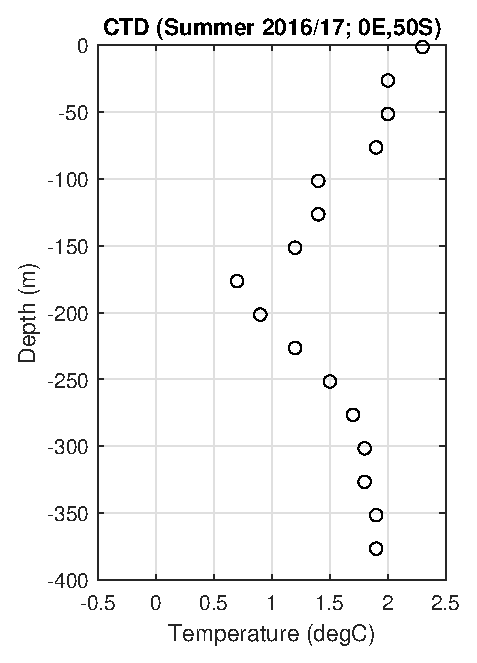
\includegraphics[scale=0.5]{figures/CTD-GHL-point}\end{onlyenv}
\end{columns}

\end{frame}

\begin{frame}{Numerical integration: midpoint rule}

\begin{columns}[t]


\column{8cm}
\begin{itemize}
\item <1->{\small{}Numerical integration is an approximate solution to
the exact integral and the only way to handle real data}{\small\par}
\item <2->The midpoint rule is the simplest method (usually with constant
depth intervals)
\end{itemize}

\column{6cm}

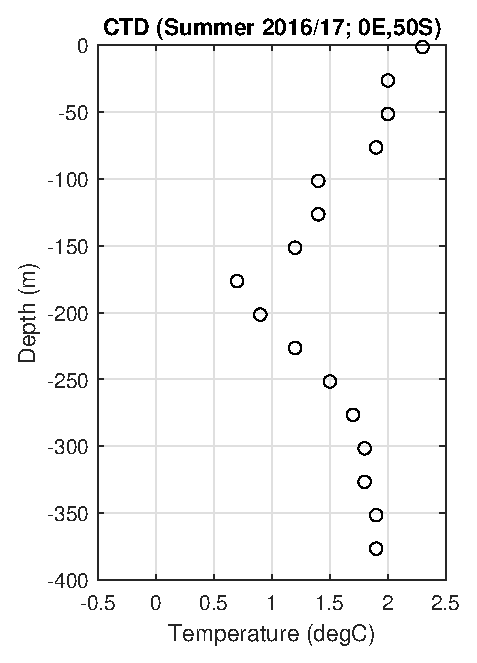
\includegraphics[scale=0.5]{figures/CTD-GHL-point}
\end{columns}

\end{frame}

\begin{frame}{Numerical integration: trapezoidal rule}

\begin{columns}[t]


\column{8cm}
\begin{itemize}
\item <2->The most generic approximation is to use the \emph{trapezoidal
rule}
\[
\int_{A}^{B}f\left(z\right)dz\approx\sum_{k=1}^{N-1}\Delta x_{k}\frac{F_{k}+F_{k+1}}{2}
\]
\item <3->But what to do at the edges? 
\item <4->More sophisticated integration methods can be used
\end{itemize}

\column{6cm}

\begin{onlyenv}<1->\includegraphics[scale=0.5]{figures/CTD-GHL-patch}\end{onlyenv}
\end{columns}

\end{frame}

\begin{frame}{Energy transfer is obtained through circulation}

\begin{itemize}
\item <1->The solar input drives the oceanic circulation through the atmosphere.
Both are affected by the Earth rotation. Energy (momentum) is transferred
from winds to the upper layers of the ocean through \textbf{frictional
coupling} between the ocean and the atmosphere at the sea surface
\item <2->The Sun also drives ocean circulation by causing variations in
the temperature and salinity of seawater which in turn control its
density. These processes drive the \textbf{thermohaline circulation}.
Changes in temperature are caused by fluxes of heat across the air-sea
boundary; changes in salinity are due to evaporation and precipitation,
but also, in polar regions, by the freezing and melting of ice. 
\item <3->All of these processes are linked directly or indirectly to the
effect of solar radiation and the related \textbf{heat and momentum
fluxes} at the surface. (suggested reading: Ocean Circulation, Open
University)
\end{itemize}
\end{frame}

\begin{frame}{Energy transport in the Earth system}

\begin{columns}[t]


\column{5cm}
\begin{itemize}
\item {\footnotesize{}The }\textbf{\footnotesize{}engine}{\footnotesize{}
of the Earth system is the }\textbf{\footnotesize{}Sun }{\footnotesize{}and
the Earth is in}\textbf{\footnotesize{} energy balance}{\footnotesize\par}
\item {\footnotesize{}The }\textbf{\footnotesize{}large scale circulation}{\footnotesize{}
of the ocean and atmosphere can be described by applying physical
principles of }\textbf{\footnotesize{}geophysical fluid dynamics}{\footnotesize{}
(3rd year)}{\footnotesize\par}
\end{itemize}

\column{9cm}

\includegraphics[width=8.3cm]{figures/heat-redistribution}
\begin{itemize}
\item \textbf{\footnotesize{}Heat is transported}{\footnotesize{} from the
equator to the poles through a network of atmospheric cells and ocean
currents}{\footnotesize\par}
\end{itemize}
\end{columns}

\end{frame}

\begin{frame}{Heat transport}

\includegraphics[scale=0.4]{figures/heat_transport}
\begin{itemize}
\item {\scriptsize{}The required total heat transport in PW ($10^{15}$
W, black line), needed to balance the net radiation imbalance at the
top of the atmosphere. This is partitioned in the oceanic (blue) and
atmospheric (red) contributions, accompanied with the associated uncertainty
range (shaded). A positive value of the transport on the x axis corresponds
to a northward transport. Figure from Fasullo and Trenberth (2008)}{\scriptsize\par}
\end{itemize}
\end{frame}

\begin{frame}{Annual net heat flux {[}W m$^{2}${]} and oceanic heat transport {[}PW{]}}

\begin{center}
\includegraphics[scale=0.35]{figures/netflux+transport}
\par\end{center}

{\tiny{}Data are from the NOCS climatology (Grist and Josey, 2003).
Superimposed numbers and arrows are the meridional heat transports
(PW) calculated from ocean velocities and temperatures, based on Bryden
and Imawaki (2001) and Talley (2003).  Heat is transported polewards
in the Pacific and Indian oceans but it is only northward in the Atlantic.
Oceanographers were puzzled by this finding (\textquotedblleft flew
in the wrong direction\textquotedblright ) There is such a substantial
loss of heat in the Arctic and North Atlantic that affects the whole
(volume) circulation creating a basin scale }\textbf{\tiny{}overturn
(Atlantic Meridional Overturning Circulation)}{\tiny\par}
\end{frame}
%
\begin{frame}{Summary of Section 3: Earth energy balance}
\begin{itemize}
\item <2->The ES is currently imbalanced in respect to the heat budget
as a result of the human-induced changes in atmospheric composition
\item <3->The radiative budget and the use of blackbody laws allow to estimate
the planetary temperature. This is modulated by the presence of greenhouse
gases and likely by the homeostasis of the living components in the
ES. Mean surface temperature has increased since pre-industrial era
\item <4->Refreshed the concept of integrals, which are essential to estimate
inventories. Learned how to compute numerical integrals
\item <5->Heat is transferred between the ES components following a latitudinal
pattern. Learned various types of surface ocean heat fluxes and parameterizations.
The ocean stored the majority of this energy imbalance in the form
of heat content. Ocean heat transport is from the equator to the poles
in all basins but the Atlantic (only northward), due to the large
heat losses in the sub-polar NA
\end{itemize}
\end{frame}


\end{document}
